\documentclass[aps,prd,twocolumn,superscriptaddress,preprintnumbers,floatfix,nofootinbib]{revtex4-2}

\usepackage{showyourwork}
\usepackage{amsfonts,amssymb,amsmath}
\usepackage{hyperref}

\definecolor{rb4}{HTML}{27408B}
\newcommand{\kw}[1]{{\color{rb4}[KW: #1 ]}}

\begin{document}

\title{Constraining gravitational wave amplitude birefringence with GWTC-3}

\author{Thomas C. K. Ng}
\email{thomas.ng@link.cuhk.edu.hk}
\affiliation{Department of Physics, The Chinese University of Hong Kong, Shatin, Hong Kong}

\author{Maximiliano Isi}
\email{misi@flatironinstitute.org}
\affiliation{Center for Computational Astrophysics, Flatiron Institute, 162 5th Ave, New York, NY 10010, United States}

\author{Kaze W. K. Wong}
\email{kwong@flatironinstitute.org}
\affiliation{Center for Computational Astrophysics, Flatiron Institute, 162 5th Ave, New York, NY 10010, United States}

\author{Will M. Farr}
\email{wfarr@flatironinstitute.org}
\affiliation{Center for Computational Astrophysics, Flatiron Institute, 162 5th Ave, New York, NY 10010, United States}
\affiliation{Department of Physics and Astronomy, Stony Brook University, Stony Brook NY 11794, United States}

\date{\today}

\begin{abstract}
    One of the major problems physicists face nowadays is that Einstein's theory of general relativity (GR) does not agree with quantum theories at some length scales.
    In recent decades, theorists have worked on many beyond-GR theories to unify both.
    Some of these theories, such as Chern-Simons gravity, suggest that there is gravitational wave (GW) amplitude birefringence.
    In our study, we perform parameter estimation (PE) to constrain the strength of GW amplitude birefringence.
    Compared to previous studies, we performed PE on more events, including events in the third LIGO-Virgo catalog (GWTC-3), and used a more realistic birefringence model to describe the phenomenon.
    We obtained a constraint tighter than previous studies for an order of magnitude.
\end{abstract}

\maketitle

\section{Introduction}
\label{sec:Introduction}
% Motivation
Since Einstein proposed his theory of general relativity (GR), it has been tested in various length scales.
After a century, we know that GR does not agree with quantum theories at some length scale.
To unify both theories, we need to study the possibility of different beyond-GR theories.
\kw{I think now it kind of goes into birefringence too fast.
Maybe talk about what effect one may expect to see in GW, in general, a bit?
Say there is polarization modification, phasing modification, etc.}
Some beyond-GR theories, such as Chern-Simons gravity, suggest that there is gravitational wave (GW) amplitude birefringence, while GR predicts no birefringence.
GW amplitude birefringence is a property of space-time that consists of the enhancement of one GW polarization over the other during wave propagation.

% Previous studies
Previous studies have constrained amplitude birefringence by performing different statistical analyses.
In \citet{Okounkova_2022}, they considered the distribution of observed inclination of the GW events in GWTC-2, the second GW transient catalog, and used the distribution to constrain the amplitude birefringence effect with the assumption of frequency independence in GW amplitude birefringence.
In \citet{Yamada_2020} and \citet{Wang_2021}, they both performed parameter estimation (PE) on the events in GWTC-1, the first GW transient catalog.

% What's new?
In this study, we used a birefringence model with higher-order terms, including amplitude birefringence's frequency dependence.
This model is more realistic than the frequency-independent model used in \citet{Okounkova_2022}.
Compared to previous studies, we also performed PE on more events, including events in GWTC-3, the third GW transient catalog.
We included 69 binary black hole merger events with the lowest false alarm rate $\leq1\mathrm{yr^{-1}}$.
These events are also listed in TABLE I in \citet{GWTC_3_population}.\footnote{
GW190720 and GW200129 are included in the list in \citet{GWTC_3_population}, but we did not include them in this study.
Details in Discussion.}

% Section guide
In Sec.~\ref{sec:Method}, we describe the modification we made to the waveform model, mention the configuration we used in the PE and show the method we used to obtain the population constraint on GW amplitude birefringence.
In Sec.~\ref{sec:Results}, we present the population constraint on GW amplitude birefringence we obtained and show the results of individual PE.
In Sec.~\ref{sec:Discussion}, we discuss the limitation of this study and provide suggestions for future studies.

\section{Method}
\label{sec:Method}
% GW polarization
GW consists of two independent polarization modes similar to electromagnetic waves, which we can represent in either the linear basis (i.e. $+$ and $\times$) or the circular basis (i.e. left-handed and right-handed).
They are related by
\begin{equation}
    h_{\mathrm{L/R}} = \frac{h_+ \pm i h_\times}{\sqrt{2}}\,,
\end{equation}
where $h_{\mathrm{L/R}}$ are the amplitude of the left-handed and right-handed polarization of the waveform, $h_+$ and $h_\times$ are the amplitude of the plus and cross polarization of the waveform.

% Waveform modification
GW amplitude birefringence would enhance one polarization mode over the other.
According to \textbf{[modification reference]}, we modified the waveform model by
\begin{equation}
    h_\mathrm{L/R}^{\mathrm{br}}=
    h_\mathrm{L/R}^{\mathrm{GR}}\times
    \exp\left(\pm\kappa\frac{d_C}{1\mathrm{Gpc}}\frac{f}{100\mathrm{Hz}}\right)\,,
    \label{eq:waveform_modification}
\end{equation}
where $h_\mathrm{L/R}^{\mathrm{br}}$ is the amplitude of the modified waveform with amplitude birefringence, $h_\mathrm{L/R}^{\mathrm{GR}}$ is the amplitude of the waveform as GR predicts, $\kappa$ is the dimensionless opacity parameter that represents the strength of the birefringence, $d_C$ is the comoving distance to the source, and $f$ is the frequency of the waveform.
We assume the modification at the source is small, which means the exponent in equation \ref{eq:waveform_modification} has to be small.
As a result, we treat the binary generates GWs as GR predicts.

Although the modification at the source is small, the effect accumulates as the GW propagates.
As the GWs propagate, the effect of birefringence will be built up with the number of cycles which depends on the distance traveled and the frequency of the GWs.
According to equation \ref{eq:waveform_modification}, a positive $\kappa$ means the left-handed polarization is enhanced over the right-handed polarization, while a negative $\kappa$ means the opposite.
Note that when $\kappa=0$, the waveform is the same as GR predicts.

% Effect on inclination PE results
In GR, the amplitude ratio of the left-handed and right-handed polarizations only depends on the inclination for a nonprecessing binary.
The relationship between the amplitude ratio and the inclination is
\begin{equation}
    \frac{h_\mathrm{L}}{h_\mathrm{R}}=\left(\frac{1-\cos\iota}{1+\cos\iota}\right)^2\,,
\end{equation}
where $\iota$ is the inclination, the angle between our line of sight and the orbital angular momentum of the binary.
The waveform modification by the birefringence effect changes the ratio of the left-handed and right-handed polarization of the waveform.
Thus, the birefringence effect will affect the PE result on $\iota$.

With the modification we implemented, the amplitude ratio of the left-handed and right-handed polarizations becomes 
\begin{equation}
    \frac{h_\mathrm{L_{obs}}}{h_\mathrm{R_{obs}}}=\frac{\left(1-\cos\iota\right)^2}{\left(1+\cos\iota\right)^2}\exp\left({2\kappa\frac{d_C}{1\mathrm{Gpc}}\frac{f}{100\mathrm{Hz}}}\right)\,,
    \label{eq:modified_amplitude_ratio}
\end{equation}
where $h_\mathrm{L_{obs}}$ and $h_\mathrm{R_{obs}}$ are the observed amplitude of left-handed and right-handed polarizations of the GWs.
As the amplitude ratio does not only depends on $\iota$ with this modification but also $\kappa$ and $d_C$, the PE results on $\iota$ and $d_C$ are affected.

In \citet{Okounkova_2022}, they assume the effect of birefringence is independent of the frequency, which is a zeroth-order approximation of the birefringence model in Chern-Simons gravity.
This assumption would create a degeneracy between $\kappa$ and $\iota$, as they can affect the amplitude ratio similarly.
To reconstruct the amplitude ratio from the interferometer data, an $\iota$ representing a more face-off inspiral can pair with a positive $\kappa$, or an $\iota$ representing a more face-on inspiral with a negative $\kappa$.
% As a result, degeneracy between $\iota$ and $\kappa$ is formed with frequency independence.

In contrast, we included the frequency dependence in the equation \ref{eq:modified_amplitude_ratio}, which is a first-order approximation of the birefringence model.
The frequency dependence can break the degeneracy between $\kappa$ and $\iota$, as this would make the effect of the birefringence affect the amplitude ratio differently compared to $\iota$.
To illustrate the frequency dependence of amplitude birefringence, the observed amplitudes of two polarizations of a simulated GW signal are shown in figure \ref{fig:birefringence}.

\begin{figure}[h]
    \script{birefringence.py}
    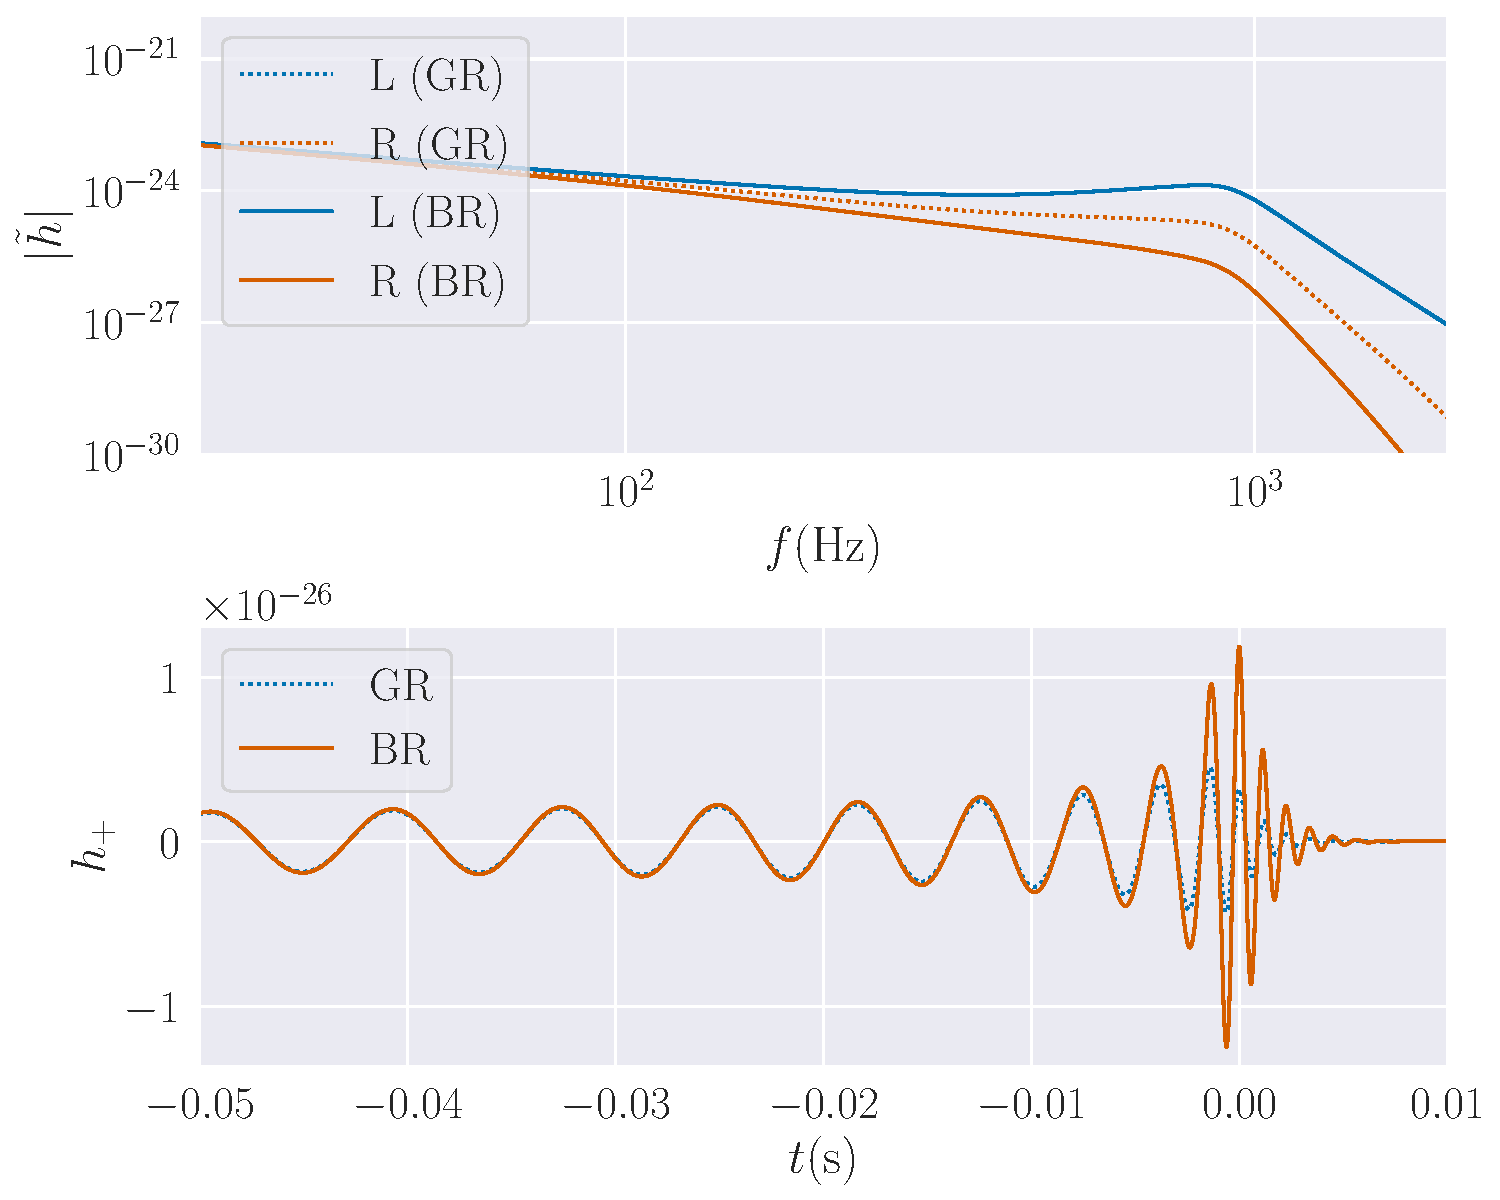
\includegraphics[width=\columnwidth]{figures/birefringence.pdf}
    \caption{
        The observed Fourier amplitude of two polarizations of a simulated GW signal with and without birefringence.
        The amplitudes, as GR predicts, are shown in dotted lines with blue and orange colors representing the left-handed and right-handed polarizations.
        The amplitudes with birefringence are shown in solid lines with blue and orange colors representing the left-handed and right-handed polarizations.
        This plot shows the effect of amplitude birefringence with frequency dependence.
    }
    \label{fig:birefringence}
\end{figure}

% Parameter estimation
To constrain $\kappa$, we perform PE with data from the third GW transient catalog \citep{GWTC-2.1, GWTC-3}, GWTC-3, using Bilby, a Bayesian toolkit for GW data analysis which can calculate posteriors of GW parameters based on interferometer data and priors for the parameters in question \citep{Bilby}.
We set the prior on $\kappa$ to a uniform distribution between $-1$ and $1$, and perform PE using the modified waveforms.
We use the same PE configuration as in \citet{GWTC-2.1, GWTC-3} for each event.
We also perform a sanity test to check if our PE could recover the PE results done by LIGO-Virgo-KAGRA Collaboration (LVK) in \citet{GWTC-2.1, GWTC-3}.
To implement the sanity check, we need to assume there is no birefringence by setting the prior on $\kappa$ to be a $\delta$ function at $0$, which force the PE results to be consistent with GR.
These sanity tests result can be found in the \href{https://zenodo.org/record/7338924}{data release}.

% Bayesian Hierarchical Modeling
With the PE results of the individual events, we can perform Bayesian hierarchical modeling to constrain the birefringence effect.
We treated $\kappa$ posteriors from all events as a set of measured $\kappa$ from an underlying distribution.
The underlying distribution can be assumed to be a Dirac delta function, which means there is a single true value of $\kappa$, or other distributions, which means there is a range of plausible values of $\kappa$.
In this study, we assume the underlying distribution is a Gaussian distribution with mean $\mu$ and standard deviation $\sigma$.
\kw{explain why we chose Gaussian}
With Bayesian hierarchical modeling, which is a method to combine multiple measurements of a random variable by assuming the measurements are independent and identically distributed, we can calculate the posterior of $\mu$ and $\sigma$ from the set of measured $\kappa$ posterior.
The posterior of $\mu$ and $\sigma$ can be calculated by
\begin{equation}
    P(\mu,\sigma|\{d_i\})\propto P(\mu,\sigma)\prod_{i}\int\frac{P(\kappa|d_i)}{P(\kappa)}P(\kappa|\mu,\sigma)\,d\kappa\,,
    \label{eq:posterior_of_mu_sigma}
\end{equation}
where function $P$ is the probability density function, and $\{d_i\}$ is the set of GW event data.
Note that $P(\kappa)$ is the prior on $\kappa$, which is a uniform distribution between $-1$ and $1$ in this study.
We chose the prior of $\mu$ and $\sigma$ being uniform distributions.
Equation \ref{eq:posterior_of_mu_sigma} can then be simplified to
\begin{equation}
    P(\mu,\sigma|\{d_i\})\propto\prod_{i}\int P(\kappa|d_i)\mathcal{N}(\mu,\sigma)\,d\kappa\,.
\end{equation}
To sample the posterior distribution of $\mu$ and $\sigma$, we used a generic sampling package, flowMC \citep{flowMC}.
We then calculate the population constraint on $\kappa$ from the posterior of $\mu$ and $\sigma$.
The constraint was calculated by
\begin{equation}
    P(\kappa|\{d_i\})=\int \mathcal{N}(\mu,\sigma)P(\mu,\sigma|\{d_i\})\,d\mu\,d\sigma\,.
\end{equation}

\section{Results}
\label{sec:Results}
In this section, we present the results of our study.
We first show the PE results of all events and present the results of Bayesian hierarchical modeling.
Then, we will discuss some special events individually.

\subsection{Result on GWTC-3}
% Stacked kappa posterior plot
In figure \ref{fig:kappa_stacked}, we show the individual posterior of $\kappa$ of each event obtained from PE.
The posteriors of $\kappa$ for most events are concentrated around $0$, which means the PE results are consistent with GR.
With Bayesian hierarchical modeling, these posteriors are used to calculate the population constraint on $\kappa$.

\begin{figure}[h]
    \script{kappa_stacked.py}
    \includegraphics[width=\columnwidth]{figures/kappa_stacked.pdf}
    \caption{
        The posterior of $\kappa$ for all 69 events included in this study.
        Each color represents a different event.
    }
    \label{fig:kappa_stacked}
\end{figure}

% Corner plot of the mean and standard deviation of kappa
The posterior of $\mu$ and $\sigma$ are shown in figure \ref{fig:corner_Gaussian}.
The mean of $\mu$ and $\sigma$ are \variable{output/Gaussian_mean.txt}, respectively.
The posterior of $\mu$ is concentrated around $0$, which means the population constraint on $\kappa$ is consistent with GR.

\begin{figure}[h]
    \script{corner_Gaussian.py}
    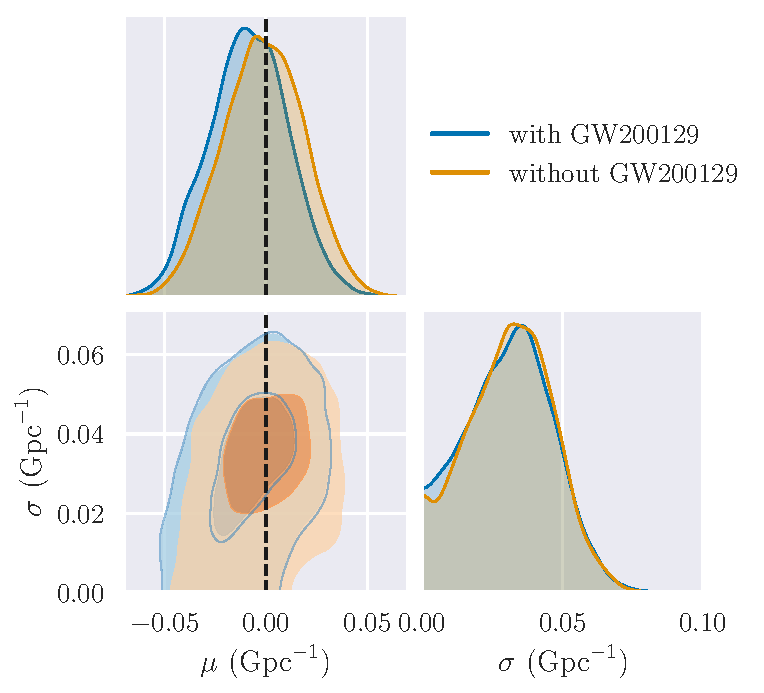
\includegraphics[width=\columnwidth]{figures/corner_Gaussian.pdf}
    \caption{
        The posterior of $\mu$ and $\sigma$ of the population distribution of $\kappa$.
        2D contour plot shows $39.35\%$ and $90\%$ confidence level.
        The orange line represents the median of $\mu$ and $\sigma$.
        The plot shows that the population constraint on $\kappa$ is consistent with GR.
    }
    \label{fig:corner_Gaussian}
\end{figure}

% Constraint on $\kappa$
With the posteriors of $\mu$ and $\sigma$, the population constraint on $\kappa$ was calculated.
The mean of the population distribution of $\kappa$ is \variable{output/kappa_mean.txt}.
Note that the result is consistent with GR when $\kappa=0$.

% Comparison with previous studies
In \citet{Okounkova_2022}, the authors gave a constraint on GW amplitude birefringence by performing statistical analysis on GWTC-2.
We convert the constraint to the same format as ours to make a comparison.
They were able to constrain $\kappa$ to be $|\kappa| \lesssim 0.74$ at $1 \sigma$.
We obtained a tighter constraint on $\kappa$ with $|\kappa| \lesssim 0.04$ at $1 \sigma$.
Our result is an order of magnitude improvement in constraining $\kappa$.
The main reason is that we have more events from GWTC-3 than GWTC-2.

% Violin plot
In figure \ref{fig:violin_kappa}, we show the posterior of $\kappa$ for each event in the form of a violin plot.
Some events with $\kappa$ distribution deviate from $\kappa=0$.
Also, there are some events with bimodal $\kappa$ distribution.
We are going to discuss some of these events in the following.

\begin{figure*}[ht]
    \script{violin_kappa.py}
    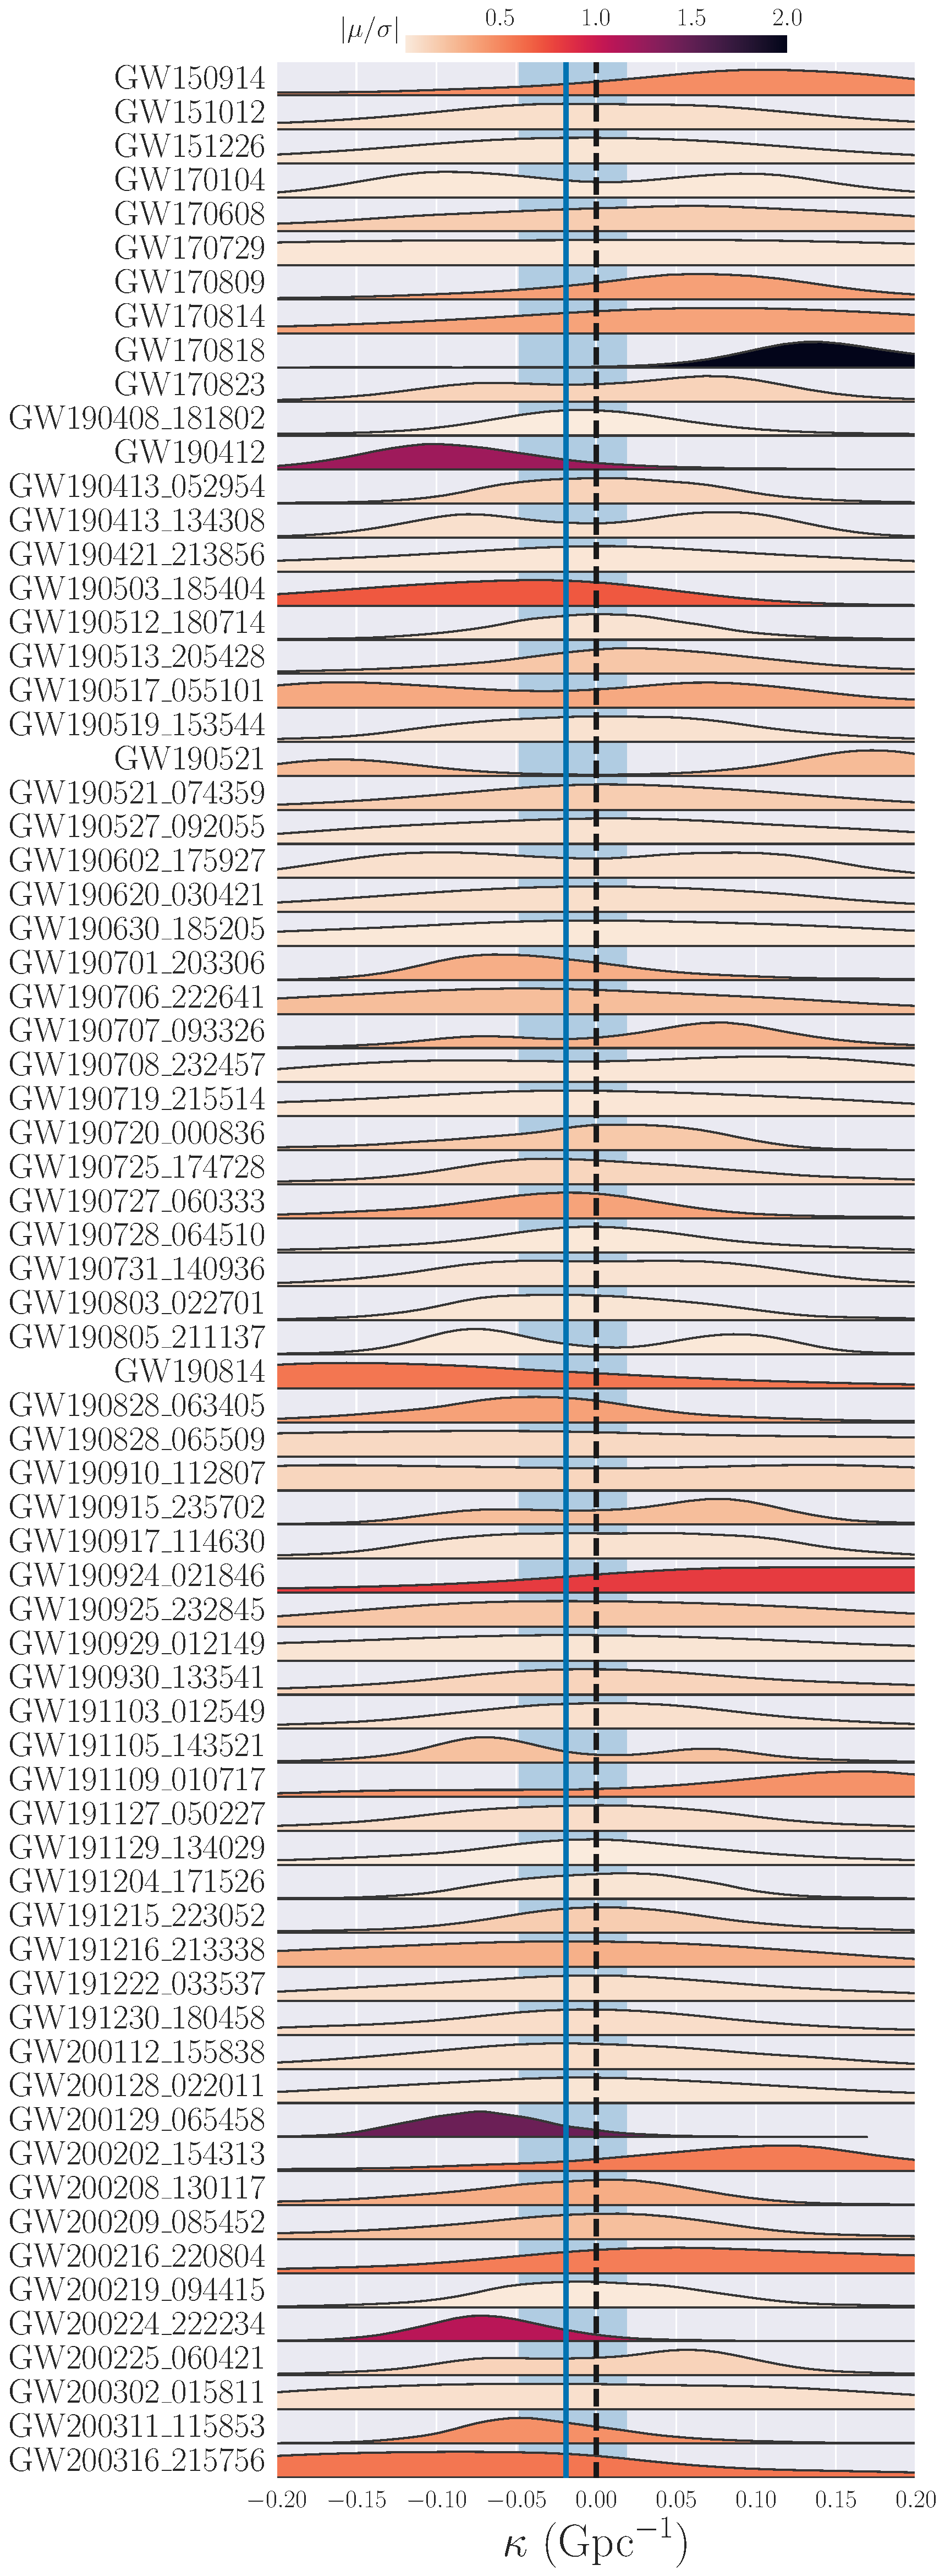
\includegraphics[width=\textwidth]{figures/violin_kappa.pdf}
    \caption{
        The violin plot shows the posterior of $\kappa$ for all 69 events in this study.
        Each violin represents a different event.
        The violins are sorted by the quotient of the median and standard deviation of the posterior.
        The blue horizontal line represents the median value of $\mu$, and the blue region represents 1 $\sigma$ confidence level.
        The Orange horizontal line represents $\kappa=0$.
        This plot shows that some events with $\kappa$ distribution significantly deviate from $0$.
    }
    \label{fig:violin_kappa}
\end{figure*}

% Trend (mass & distance)

% Constraining power

% Case study
% Case: GW170818

% Case: GW150914 (example of broken degeneracy)
\subsection{Result on GW150914}
In this study, we included frequency dependence of birefringence, which would affect the posterior of $\kappa$ obtained from PE.
Consider GW150914, the first GW detected by LIGO, as an example.
In figure \ref{fig:corner_GW150914}, we show the posteriors of the parameters of GW150914.
With the frequency-independent birefringence model, the posteriors for $\cos\iota$ look different from the posteriors assuming GR.
This is because, for a nonprecessing system, there is a degeneracy between $\kappa$ and $\iota$ if the frequency dependence is not included.
\kw{you should say why the middle part is constrained to be small.}

On the other hand, with the frequency-dependent birefringence model, the posterior looks similar to the GR posterior.
This is because the frequency dependence broke the degeneracy, as the effect of birefringence will differ from the effect of changing $\iota$.
In this case, the most probable value of $\kappa$ is close to $0$, which means the birefringence is weak or absent.
Therefore, the PE result with frequency dependence is consistent with GR.

\begin{figure}[h]
    \script{corner_GW150914.py}
    \includegraphics[width=\columnwidth]{figures/corner_GW150914.pdf}
    \caption{
        The posterior of $\kappa$, luminosity distance $d_L$ and $\cos{\iota}$ for GW150914.
        Colors in the plot represent the PE result with GR done by LVK without cosmological reweighing \citep{GWTC-2.1, GWTC-3}, the PE results done by us with both frequency independent and dependent birefringence respectively.
        2D contour plot shows $39.35\%$ and $90\%$ confidence level.
        Note that there is no posterior of $\kappa$ for the PE result from LVK, as the LVK PE is based on GR, which does not suggest GW amplitude birefringence.
        This plot shows that frequency-independent birefringence creates a degeneracy between $\kappa$ and $\iota$, while the frequency-dependent birefringence can break it.
    }
    \label{fig:corner_GW150914}
\end{figure}

% Case: GW190521 (massive BBH)
\subsection{Result on GW190521}
Even with the frequency-dependent birefringence model, some events still have a bimodal $\kappa$ distribution.
Consider GW190521, the most massive binary black hole merger in the events we included.
The degeneracy between $\kappa$ and $\iota$ cannot be broken by the frequency-dependent birefringence model, as shown in figure \ref{fig:corner_GW190521}.
The reason could be this GW event's frequency range is too narrow to break the degeneracy.
The effect of birefringence at different frequencies within the range is similar, so the degeneracy cannot be broken.
Therefore, the narrow frequency range can be a possible reason why the $\kappa$ distribution of GW190521 is bimodal.

\begin{figure}[h]
    \script{corner_GW190521.py}
    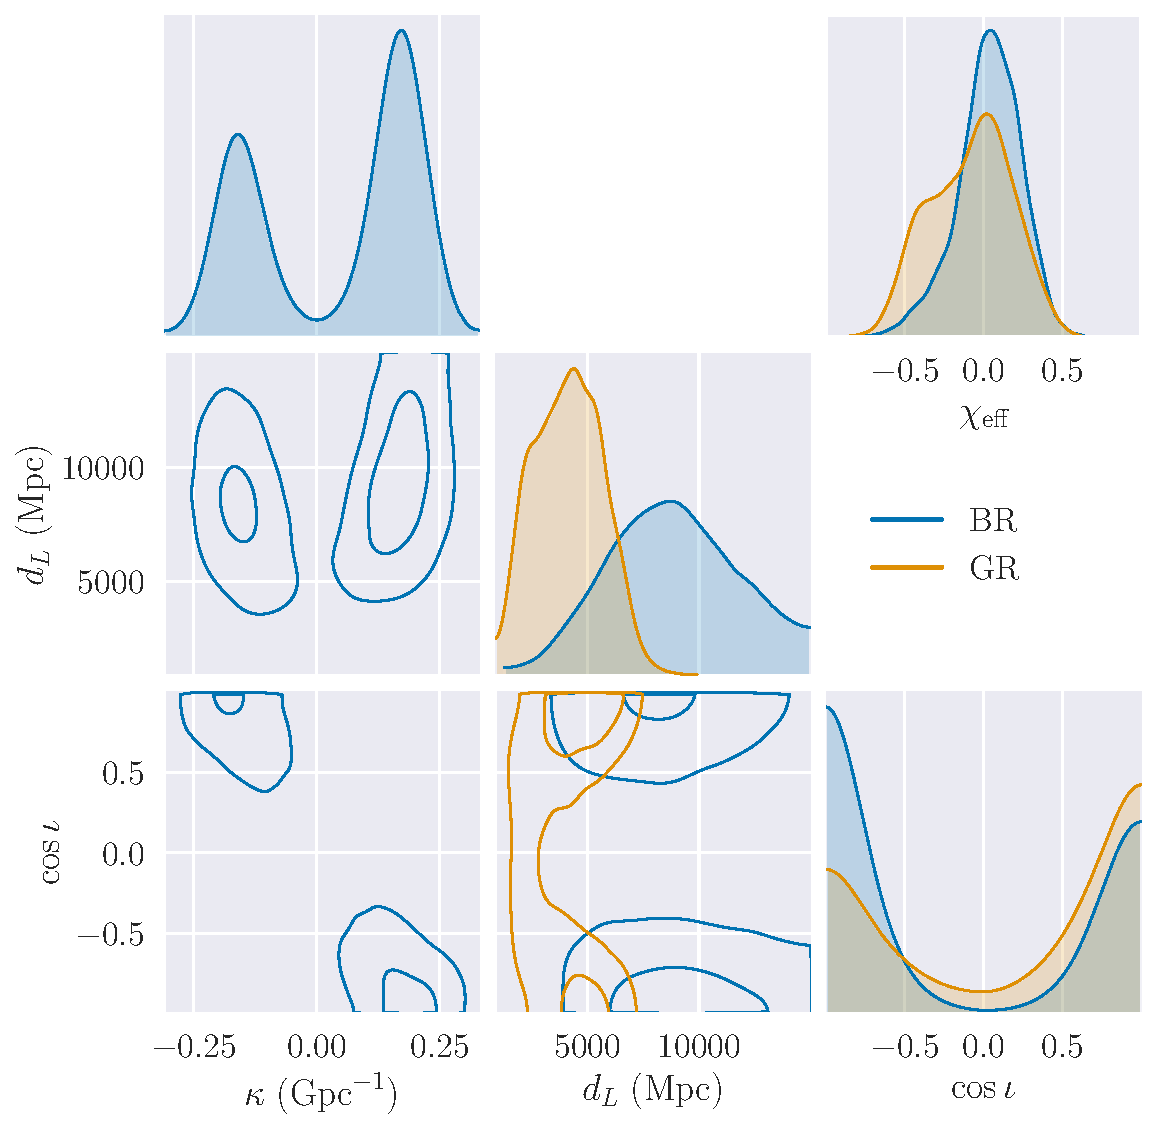
\includegraphics[width=\columnwidth]{figures/corner_GW190521.pdf}
    \caption{
        The posterior of $\kappa$, luminosity distance $d_L$ and $\cos{\iota}$ for GW190521.
        Colors in the plot are the PE result with GR done by LVK without cosmological reweighing \citep{GWTC-2.1, GWTC-3} and the PE result done by us with the frequency-dependent birefringence.
        2D contour plot shows $39.35\%$ and $90\%$ confidence level.
        This plot shows that frequency-dependent birefringence cannot break the degeneracy between $\kappa$ and $\iota$.
    }
    \label{fig:corner_GW190521}
\end{figure}

\section{Discussion}
\label{sec:Discussion}

% Reasons for special events
\subsection{Special Events}
% Special event 1: GW190720
For GW190720, we could not perform PE with Bilby successfully.
In LVK PE papers \citep{GWTC-2.1, GWTC-3}, the PE of some events was performed with LALInference \citep{lalsuite} instead of Bilby.
GW190720 was one of them.
We successfully migrated the LALInference configuration to Bilby for most of these events and recovered similar PE results, except for GW190720.
Bilby could not evaluate the likelihood function on Virgo data.
As a result, we excluded this event from our analysis.

% Special event 2: GW200129
For GW200129, past research suggests a potential glitch in Virgo data. \citep{GW200129}
We perform three sets of PE to check if the glitch would affect the population posterior of $\kappa$.
We pick only two out of three detector data in each set to perform PE.
The two sets of PE results with Virgo data return a $\kappa$ posterior that strongly suggests a negative $\kappa$.
Further investigation is needed to understand the glitch.
Thus, we did not include this event in our analysis.

% Future work
\subsection{Future Work}
% BNS
Future work is to perform PE on binary neutron star mergers, such as GW170817.
The frequency range of the signal is much wider compared to the binary black hole mergers.
Thus, the difference in the effect of birefringence at different frequencies within the range can be more significant.
The PE on binary neutron star mergers can allow us to further constrain the birefringence effect and the beyond-GR theories that predict it.
However, performing PE on binary neutron star mergers requires much more computational resources.
Therefore, we may need to wait for future PE methods and tools to further our work.

% More observations with higher SNR
Another future work is to apply the same method to more GW events and events with a higher signal-to-noise ratio (SNR).
LVK will release more events with higher SNR in the future.
Using data with higher SNR allows us to obtain more precise PE results and constrain the birefringence effect more precisely.
And using data from more events will allow us to calculate a more constrained population posterior of $\kappa$.

\section{Acknowledgements}
\label{sec:Acknowledgements}
M.~I., K.~W.~K.~W.~, and W.~M.~F.~ are funded by the Center for Computational Astrophysics at the Flatiron Institute.
The Flatiron Institute provided the computational resources used in this work.

\bibliography{bib}

\end{document}
